\section{离散信号的傅里叶变换}

本节讨论离散信号的傅里叶变换(Discrete-Time Fourier Transform,DTFT)。
相应地,连续信号的傅里叶变换称为Continuous-Time Fourier Transform,CTFT。
本节是向离散傅里叶变换(Discrete Fourier Transform,DFT)的过渡。

本节要点:
\begin{itemize}
    \item 掌握DTFT;
    \item 熟悉CTFT和DTFT的关系;
    \item 理解采样周期对DTFT的影响。
\end{itemize}

%============================================================
\subsection{DTFT的概念}

\begin{definition}[离散信号的傅里叶变换]
我们已知连续信号$x\left( t \right) $的傅里叶变换
\begin{align*}
&X\left( \omega \right) =\int_{-\infty}^{+\infty}{x\left( t \right) e^{-i\omega t}dt} \\
&x\left( t \right) =\frac{1}{2\pi}\int_{-\infty}^{+\infty}{X\left( \omega \right) e^{i\omega t}d\omega}
\end{align*}
同样我们可以定义,若离散信号$x\left[ n \right] $满足:
\begin{itemize}
    \item 任一有限区域上满足狄利克雷收敛条件,
    \item 整个实数域绝对可积,即$\sum_{n=-\infty}^{+\infty}{\left| x\left[ n \right] \right|}$收敛,
\end{itemize}
则有:
\[
x\left[ n \right] =\frac{1}{2\pi}\int_0^{2\pi}{\left[ \sum_{n=-\infty}^{+\infty}{x\left[ n \right] e^{-i\varOmega n}} \right] e^{i\varOmega n}d\varOmega}
\]
同时称$\sum_{n=-\infty}^{+\infty}{x\left[ n \right] e^{-i\varOmega n}}$为{\bf 离散信号$x\left[ n \right] $的傅里叶变换}(Discrete-Time Fourier Transform,DTFT),记为$X\left( \varOmega \right) $,即:
\[
X\left( \varOmega \right) =\sum_{n=-\infty}^{+\infty}{x\left[ n \right] e^{-i\varOmega n}}
\]
相应地称
\[
x\left[ n \right] =\frac{1}{2\pi}\int_0^{2\pi}{X\left( \varOmega \right) e^{i\varOmega n}d\varOmega}
\]
为{\bf 离散信号的傅里叶逆变换}。离散信号的傅里叶变换形式通常记为:
\[
x\left[ n \right] \overset{\mathscr{F}}{\leftrightarrow}X\left( \varOmega \right)
\]
\end{definition}

\begin{tcolorbox}
注意,为区别连续信号,离散信号的傅里叶变换的自变量通常用大写$\varOmega $表示。
其次,$X\left( \varOmega \right) $依然是连续函数。
\end{tcolorbox}

%============================================================
\subsection{DTFT的量纲}

从定义看,信号的离散化使得$n$的量纲是时间,且有$\Delta n=n-\left( n-1 \right) =1$,于是:
\[
X\left( \varOmega \right) =\sum_{n=-\infty}^{+\infty}{\left\{ x\left[ n \right] e^{-i\varOmega n}\cdot \Delta n \right\}}
\]
易得$X\left( \varOmega \right) $的量纲依然是信号的量纲除以频率的量纲$\mathrm{D}_x\cdot \mathrm{Hz}^{-1}$,和CTFT一样。
这点从逆变换形式更好理解。

$\varOmega $的量纲和$\omega $一致,表示角频。
\begin{align*}
&\because \begin{cases}
	\omega \cdot t=s\\
	\varOmega \cdot n=\varOmega \cdot \frac{t}{T_{sample}}=s\\
\end{cases} \\
&\therefore \varOmega =\omega \cdot T_{sample}=\frac{\omega}{f_{sample}}
\end{align*}
其中$s$表示弧长。
可以认为$\varOmega $和$\omega $差了一个采样频率,相当于通过$T_{sample}$做了一个尺度变换。

%============================================================
\subsection{DTFT的极坐标形式}

DTFT可以变成极坐标形式:
\begin{align*}
X\left( \varOmega \right) &=\sum_{n=-\infty}^{+\infty}{x\left[ n \right] e^{-i\varOmega n}} \\
&=\sum_{n=-\infty}^{+\infty}{x\left[ n \right] \cos \left( n\varOmega \right)}+i\sum_{n=-\infty}^{+\infty}{-x\left[ n \right] \sin \left( n\varOmega \right)} \\
&=R\left( \varOmega \right) +iI\left( \varOmega \right)
\end{align*}
于是:
\begin{align*}
&\begin{cases}
	\left| X\left( \varOmega \right) \right|=\sqrt{R^2\left( \varOmega \right) +I^2\left( \varOmega \right)}\\
	\angle X\left( \varOmega \right) =\mathrm{arc}\tan \frac{I\left( \varOmega \right)}{R\left( \varOmega \right)}\\
\end{cases} \\
&X\left( \varOmega \right) =\left| X\left( \varOmega \right) \right|\cdot e^{i\angle X\left( \varOmega \right)}
\end{align*}
同样,DTFT的幅频是偶函数,相频是奇函数,且本身有$X\left( -\varOmega \right) =\bar{X}\left( \varOmega \right) $。

%============================================================
\subsection{广义DTFT}

对于有些函数,如$x\left[ n \right] =1$等,由于不满足绝对可积条件,没有严格意义上的DTFT,但可以通过单位冲激定义广义DTFT。

假设某信号DTFT之后有$2\pi \delta \left( \varOmega \right) $,则原信号:
\begin{align*}
&\because \frac{1}{2\pi}\int_{-\pi}^{+\pi}{2\pi \delta \left( \varOmega \right) e^{i\varOmega n}d\varOmega}=\int_{-\pi}^{+\pi}{\delta \left( \varOmega \right) e^{i\varOmega n}d\varOmega}=1 \\
&\therefore 1\overset{\mathscr{F}}{\rightarrow}2\pi \delta \left( \varOmega \right)
\end{align*}
以上只是一个例子,通过$\delta \left[ n \right] $的DTFT和DTFT的性质,我们可以求得很多函数的广义DTFT。

%============================================================
\subsection{DTFT的性质}

{\bf 奇偶性}

通过DTFT的直角坐标形式易得,如果$x\left[ n \right] $是偶函数,则其DTFT是实函数,如果$x\left[ n \right] $是奇函数,则其DTFT是纯虚函数,此外,一般DTFT是$\varOmega $的复变函数。
\begin{align*}
&x\left[ n \right] \text{ is even} \quad \Rightarrow \quad X\left( \varOmega \right) =x\left[ 0 \right] +2\sum_{n=1}^{+\infty}{x\left[ n \right] \cos \left( n\varOmega \right)} \\
&x\left[ n \right] \text{ is even} \quad \Rightarrow \quad X\left( \varOmega \right) =-2i\sum_{n=1}^{+\infty}{x\left[ n \right] \sin \left( n\varOmega \right)}
\end{align*}

{\bf 周期性}

对于任何离散信号,其DTFT都是周期函数,且$T=2\pi $。
简单证明:
\begin{align*}
X\left( \varOmega +2\pi \right) &=\sum_{n=-\infty}^{+\infty}{x\left[ n \right] e^{-i\left( \varOmega +2\pi \right) n}}=\sum_{n=-\infty}^{+\infty}{x\left[ n \right] e^{-i\varOmega n}e^{-i2\pi n}} \\
&=\sum_{n=-\infty}^{+\infty}{x\left[ n \right] e^{-i\varOmega n}}
\end{align*}
可见,DTFT的周期性源于信号的离散性。
由于$X\left( \varOmega \right) $的周期性,逆变换的积分范围可以是$\left[ 0,2\pi \right] $,也可以是$\left[ -\pi ,\pi \right] $。
加之DTFT的幅频是偶函数、相频是奇函数,所以DTFT的好处是对于信号的频域分析,只需要考察$\left[ 0,\pi \right] $即可。

{\bf 采样的频域特性}

\[
\begin{cases}
	x\left[ n \right] \leftrightarrow X\left( \varOmega \right)\\
	\gamma \left( t \right) \leftrightarrow X\left( \omega \right) p_{2\pi}\left( \omega \right)\\
\end{cases} \quad \Rightarrow \quad x\left[ n \right] =\left. \gamma \left( t \right) \right|_{t=n}=\gamma \left[ n \right]
\]

这说明所谓的采样,在频域看来就是通过一个带宽$B=\pi $的低通。
或者说,采样后信号的频域从原来的整个实数限制到$\left[ -\pi ,\pi \right] $。
简单证明:
\begin{align*}
&\because \gamma \left( t \right) =\frac{1}{2\pi}\int_{-\infty}^{+\infty}{X\left( \omega \right) p_{2\pi}\left( \omega \right) e^{i\omega t}d\omega}=\frac{1}{2\pi}\int_{-\pi}^{+\pi}{X\left( \omega \right) e^{i\omega t}d\omega} \\
&\therefore \gamma \left( n \right) =\frac{1}{2\pi}\int_{-\pi}^{+\pi}{X\left( \omega \right) e^{i\omega n}d\omega}=\frac{1}{2\pi}\int_{-\pi}^{+\pi}{X\left( \varOmega \right) e^{i\varOmega n}d\varOmega}=x\left[ n \right]
\end{align*}
上述证明过程中,$t$到$n$只是一个简单的变量替换,所以,这里的“采样”固定了周期$T=1$。
如果要获得不一样的采样周期,可以先在时域做尺度变换。

{\bf 线性性}

\[
ax\left[ n \right] +by\left[ n \right] \leftrightarrow aX\left( \varOmega \right) +bY\left( \varOmega \right)
\]

{\bf 时移性、频移性}

\begin{align*}
&x\left[ n-n_1 \right] \leftrightarrow X\left( \varOmega \right) \cdot e^{-i\varOmega n_1} \\
&e^{-i\varOmega _1n}\cdot x\left[ n \right] \leftrightarrow X\left( \varOmega -\varOmega _1 \right)
\end{align*}

{\bf 反转性}

\[
x\left[ -n \right] \leftrightarrow X\left( -\varOmega \right) =\bar{X}\left( \varOmega \right)
\]

注意,DTFT没有CTFT中的“时展性”。
或者说,DTFT的“时展性”体现在对连续信号的采样周期上。
采样周期确实对DTFT结果有影响。

{\bf 三角律}

\begin{align*}
&x\left[ n \right] \cos \varOmega _1t\leftrightarrow \frac{1}{2}\left[ X\left( \varOmega +\varOmega _1 \right) +X\left( \varOmega -\varOmega _1 \right) \right] \\
&x\left[ n \right] \sin \varOmega _1t\leftrightarrow \frac{i}{2}\left[ X\left( \varOmega +\varOmega _1 \right) -X\left( \varOmega -\varOmega _1 \right) \right]
\end{align*}

{\bf 时域和}

\[
\sum_{k=1}^n{x\left[ k \right]}\leftrightarrow \frac{1}{1-e^{-i\varOmega}}X\left( \varOmega \right) +\sum_{k=-\infty}^{+\infty}{\pi X\left( 2\pi k \right) \delta \left( \pi -2\pi k \right)}
\]

{\bf 频域的微分}

\[
\left( \frac{n}{i} \right) ^m\cdot x\left[ n \right] \leftrightarrow \frac{d^mX\left( \varOmega \right)}{d\varOmega ^m}
\]

{\bf 卷积性}

\begin{align*}
&x\left[ n \right] \ast y\left[ n \right] \leftrightarrow X\left( \varOmega \right) \cdot Y\left( \varOmega \right) \\
&x\left[ n \right] \cdot y\left[ n \right] \leftrightarrow \frac{1}{2\pi}\int_{-\pi}^{+\pi}{X\left( \varOmega -\lambda \right) Y\left( \lambda \right) d\lambda}
\end{align*}

{\bf Parseval定理}

\begin{align*}
&\sum_{n=-\infty}^{+\infty}{x\left[ n \right] y\left[ n \right]}=\frac{1}{2\pi}\int_{-\pi}^{+\pi}{\bar{X}\left( \varOmega \right) Y\left( \varOmega \right) d\varOmega} \\
&\sum_{n=-\infty}^{+\infty}{x^2\left[ n \right]}=\frac{1}{2\pi}\int_{-\pi}^{+\pi}{\left| X\left( \varOmega \right) \right|^2d\varOmega}
\end{align*}

\begin{tcolorbox}
注意,DTFT没有CTFT中的“Duality”。
\end{tcolorbox}

%============================================================
\subsection{CTFT和DTFT对比}

\begin{table}[h]
\centering
% \caption{表头}
\begin{tabular}{ccc}
    \toprule
    & CTFT & DTFT\\
    \midrule
    变换 & $X\left( \omega \right) =\int_{-\infty}^{+\infty}{x\left( t \right) e^{-i\omega t}dt}$ & $X\left( \varOmega \right) =\sum_{n=-\infty}^{+\infty}{x\left[ n \right] e^{-i\varOmega n}}$\\
    逆变换 & $x\left( t \right) =\frac{1}{2\pi}\int_{-\infty}^{+\infty}{X\left( \omega \right) e^{i\omega t}d\omega}$ & $x\left[ n \right] =\frac{1}{2\pi}\int_0^{2\pi}{X\left( \varOmega \right) e^{i\varOmega n}d\varOmega}$\\
    时域变量 & 连续时间$t$ & 离散时间$n$\\
    频域变量 & 连续频率$\omega $ & 连续频率$\varOmega \in \left[ -\pi ,\pi \right] $\\
    周期 & 无 & $T=2\pi $\\
    \bottomrule
\end{tabular}
\end{table}

%============================================================
\subsection{例}

\begin{example}
设两个信号$x\left( t \right) =0.5^tu\left( t \right) ,x\left[ n \right] =0.5^nu\left[ n \right] $,分析两者的傅里叶变换。
\end{example}

$x\left( t \right) =0.5^tu\left( t \right) $的CTFT:
\begin{align*}
X\left( \omega \right) &=\int_{-\infty}^{+\infty}{0.5^tu\left( t \right) e^{-i\omega t}dt}=\int_0^{+\infty}{\left( 0.5e^{-i\omega} \right) ^tdt} \\
&=\left. \frac{\left( 0.5e^{-i\omega} \right) ^t}{\ln \left( 0.5e^{-i\omega} \right)} \right|_{0}^{+\infty}=-\frac{1}{\ln \left( 0.5e^{-i\omega} \right)}=-\frac{1}{\ln 0.5-i\omega}
\end{align*}

$x\left[ n \right] =0.5^nu\left[ n \right] $的DTFT,为公比$\left| 0.5e^{-i\varOmega} \right|<1$的无穷等比数列的和:
\[
X\left( \varOmega \right) =\sum_{n=-\infty}^{+\infty}{x\left[ n \right] e^{-i\varOmega n}}=\sum_{n=-\infty}^{+\infty}{0.5^ne^{-i\varOmega n}}=\frac{1}{1-0.5e^{-i\varOmega}}
\]

\begin{python}
t   = np.arange(0, 5, 0.01)
x_t = 0.5**t
w   = np.arange(-3*np.pi, 3*np.pi, 0.01)
X_w = -1 / (np.log(0.5) - w*1.0j)
n   = np.arange(0,26)
x_n = 0.5**(0.2*n)
W   = np.arange(-3*np.pi, 3*np.pi, 0.01)
X_W = 1 / (1 - 0.5*np.exp(-1.0j*W))

axs[0][0].plot(t, x_t)
plot_mag_phs(w, np.abs(X_w), np.angle(X_w, deg=True), ...)
axs[0][1].stem(n, x_n)
plot_mag_phs(w, np.abs(X_W), np.angle(X_W, deg=True), ...)
\end{python}

\begin{figure}[h]
\centering
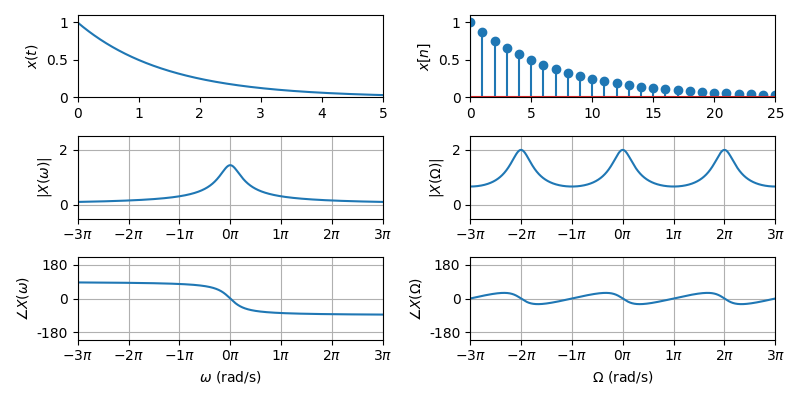
\includegraphics[height=5cm]{6.1.7-1.png}
\end{figure}

~

\begin{example}
设两个信号$x\left( t \right) =\left( -0.5 \right) ^tu\left( t \right) ,x\left[ n \right] =\left( -0.5 \right) ^nu\left[ n \right] $,(基本同上例,只是系数变成了-0.5,增强了信号波动频率),分析两者的傅里叶变换。
\end{example}

两个信号的傅里叶变换:
\begin{align*}
&\left( -0.5 \right) ^tu\left( t \right) \leftrightarrow -\frac{1}{\ln \left( -0.5 \right) -i\omega} \\
&\left( -0.5 \right) ^nu\left[ n \right] \leftrightarrow \frac{1}{1+0.5e^{-i\varOmega}}
\end{align*}

\begin{python}
t   = np.arange(0, 5, 0.01, dtype=np.complex64)
x_t = (-0.5)**t
w   = np.arange(-3*np.pi, 3*np.pi, 0.01)
X_w = -1 / (np.log(-0.5+0.0j) - 1.0j*w)
n   = np.arange(0,26, dtype=np.complex64)
x_n = (-0.5)**(0.2*n)
W   = np.arange(-3*np.pi, 3*np.pi, 0.01)
X_W = 1 / (1 + 0.5*np.exp(-1.0j*W))

axs[0][0].plot(t.real, x_t.real)
plot_mag_phs(w, np.abs(X_w), np.angle(X_w, deg=True), ...)
axs[0][1].stem(n.real, x_n.real)
plot_mag_phs(w, np.abs(X_W), np.angle(X_W, deg=True), ...)
\end{python}

\begin{figure}[h]
\centering
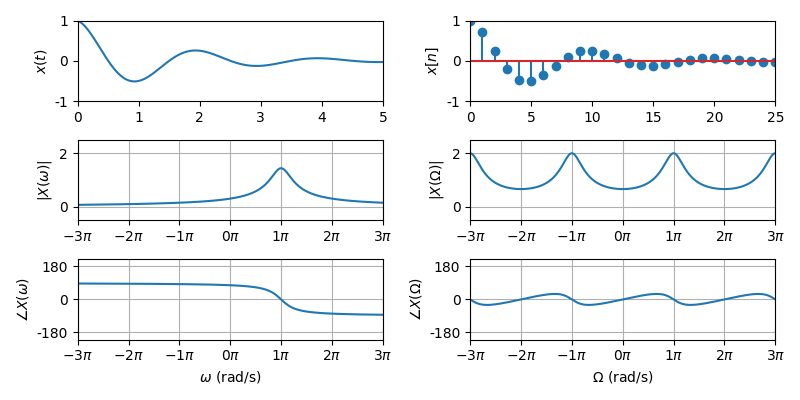
\includegraphics[height=5cm]{6.1.7-2.png}
\end{figure}

\begin{itemize}
    \item DTFT依然呈现周期性;
    \item 对比两个FT,0.5的FT集中在低频,-0.5的FT集中在高频。
\end{itemize}

%============================================================
\subsection{采样周期对DTFT的影响}

从量纲分析可得,DTFT和CTFT两者的意义相同,区别只在于变量。
由于对时域信号做了采样,所以暂时可以认为$\varOmega $对于$\omega $做了尺度变换,$\varOmega =\omega \cdot T_{sample}$。
而且通常$T_{sample}<1$,相当于信号变慢。
所以随着采样频率的提高,DTFT结果会向低频段集中。

实际上,DTFT的频率范围只是$\left[ -\pi ,\pi \right] $,其他部分都是周期性的复现。
由于对称性,实际分析的只是$\left[ 0,\pi \right] $,称为“窗口”。
DTFT在频率轴上开了一个窗口,将CTFT的频率“映射”到$\left[ 0,\pi \right] $,通过采样频率将CTFT的$0\text{~}\pi \cdot f_{sample}$部分映射到窗口中。
所以采样频率越高,我们在DTFT上看到的频率越宽广。

用前面的例子说明。
假设时域信号$x\left( t \right) =\left( -0.5 \right) ^t\cdot u\left( t \right) $,分析采样周期$T$对DTFT的影响。

令$t=nT$进行离散化,得到DTFT结果:
\begin{align*}
x\left[ n \right] &=\left( -0.5 \right) ^{nT}=\left[ \left( -0.5 \right) ^T \right] ^n \\
X\left( \varOmega \right) &=\sum_{n=-\infty}^{+\infty}{x\left[ n \right] e^{-i\varOmega n}}=\sum_{n=-\infty}^{+\infty}{\left[ \left( -0.5 \right) ^T \right] ^ne^{-i\varOmega n}} \\
&=\frac{1}{1-\left( -0.5 \right) ^Te^{-i\varOmega}}
\end{align*}
\begin{figure}[h]
\centering
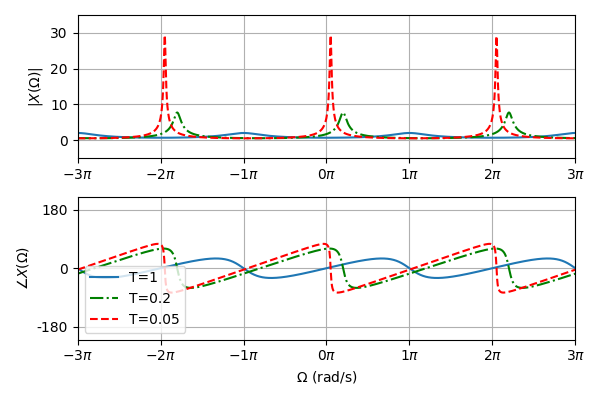
\includegraphics[height=5cm]{6.1.8-1.png}
\end{figure}

\begin{python}
W = np.arange(-3*np.pi, 3*np.pi, 0.01)
T = 1;    X_1 = 1 / (1 - (-0.5)**T * np.exp(-1.0j*W))
T = 0.2;  X_2 = 1 / (1 - (-0.5)**T * np.exp(-1.0j*W))
T = 0.05; X_3 = 1 / (1 - (-0.5)**T * np.exp(-1.0j*W))

plot_mag_phs(W, np.abs(X_1), np.angle(X_1, deg=True),
             mag_line_fmt='-', phs_line_fmt='-',
             mag_line_label='T=1', phs_line_label='T=1')
plot_mag_phs(W, np.abs(X_2), np.angle(X_2, deg=True),
             mag_line_fmt='g-.', phs_line_fmt='g-.',
             mag_line_label='T=0.2', phs_line_label='T=0.2')
plot_mag_phs(W, np.abs(X_3), np.angle(X_3, deg=True),
             mag_line_fmt='r--', phs_line_fmt='r--',
             mag_line_label='T=0.05', phs_line_label='T=0.05')
\end{python}

注意:
\begin{itemize}
    \item $T=1$时,可以认为就是原信号,即$X\left( \varOmega \right) =X\left( \omega \right) $。
    \item 随着采样频率的提高,DTFT窗口看到的频率越宽,使得“峰越往低频方向偏移”,或者认为在同样的 的“步频”下,采样频率越高信号“走得越慢”。
\end{itemize}




